\section{Evolutionnary Algorithm}
The first part of this project consisted in finding three quantities that influence the orbit of Earth around Sun: the mass of Sun, the mass of Earth and the speed of earth at the perihelion, using the evolutionnary algorithms implemented in EASEA.\\
In order to do that, we performed three distinct experiences because the sampling method does not allow us to find these three quantities simultaneously. It is impossible to find the mass of Earth and Sun at the same time because they are only bound in a product in Newton's law of universal gravitation. So there are a plethora of pair of values leading to the same result.\\
The first step consist in sampling the Earth orbit around Sun with the real quantities in order to obtain a list of polar coordinates of Earth in the heliocentric referential.\\
The genom of each individual correspond to the quantity to find (the mass or the speed) and is initialised to a value of the same order of magnitude as the real value.\\
From one generation to another, children are created by computing the mean of the two parents. Each individual can mutate with a given probability. This mutation correspond to an increase or a decrease of a given percentage of its genom.\\
The score is defined as the difference between the real orbit and the orbit with the quantity found in the genoms. That is to say: the sum of the distances between the corresponding points of the two trajectories. By doing so, the result of the algorithm does not directly depend on the value we want to find but rather on samples of coordinates that could have been made without knowing the quantity.\\
We settled for weak elitism, a form of elitism that ensures the best individual of the global population (children and parents) is conserved in the next generation.


% La première partie du sujet consistait à retrouver trois valeurs influençant l'orbite de la Terre autour du Soleil : la masse du Soleil, la masse de la Terre et la vitesse de la Terre à la périhélie en utilisant les algorithme évolutionnaires présents dans EASEA.\\
% Pour cela nous avons procédé en trois étapes distinctes car la méthode d'échantillonnage ne permet pas de retrouver les trois quantités simultanément. En effet, il n'est pas possible de retrouver la masse de la Terre et la masse du Soleil en une seule expérience car elles sont uniquement présentes dans un produit dans la formule de Newton. Il existe donc une multitude de couples de valeurs menant au même résultat.\\
% La première étape consiste à effectuer un échantillonnage avec les valeurs réelles afin d'obtenir une liste de coordonnées polaires de la Terre dans le référentiel Héliocentrique.\\
% Le génome de chaque individu correspond à la quantité à retrouver qui est initialisée à une valeur de l'ordre de grandeur attendu.\\
% D'une génération à l'autre, un individu fils correspond à la moyenne de ses deux parents et chaque individu peut muter avec une certaine probabilité. Cette mutation corrrespond à une augmentation ou une diminution d'un certain pourcentage de sa valeur.\\
% Afin de calculer le score, on procède à un nouvel échantillonnage de la position de la Terre dans le référentiel Héliocentrique avec la valeur trouvée. Dans le cas de la vitesse de la Terre à la périhélie, la vitesse trouvée est utilisée comme vitesse initiale.\\
% Le score correspond à la somme des distances entre les points des deux trajectoires ainsi obtenues. Ainsi le résultat du programme ne dépend pas directement de la valeur à trouver mais d'échantillons qui auraient pu être observés sans connaitre la quantité.\\
% Nous utilisons de l'élitisme faible, c'est à dire que le meilleur individu de la population globale (parents et enfants) est garanti d'être conservé dans la prochaine génération.

\subsection{Mass of Sun}
% \clearpage
\begin{wrapfigure}{R}{0.5\textwidth}
    \center
    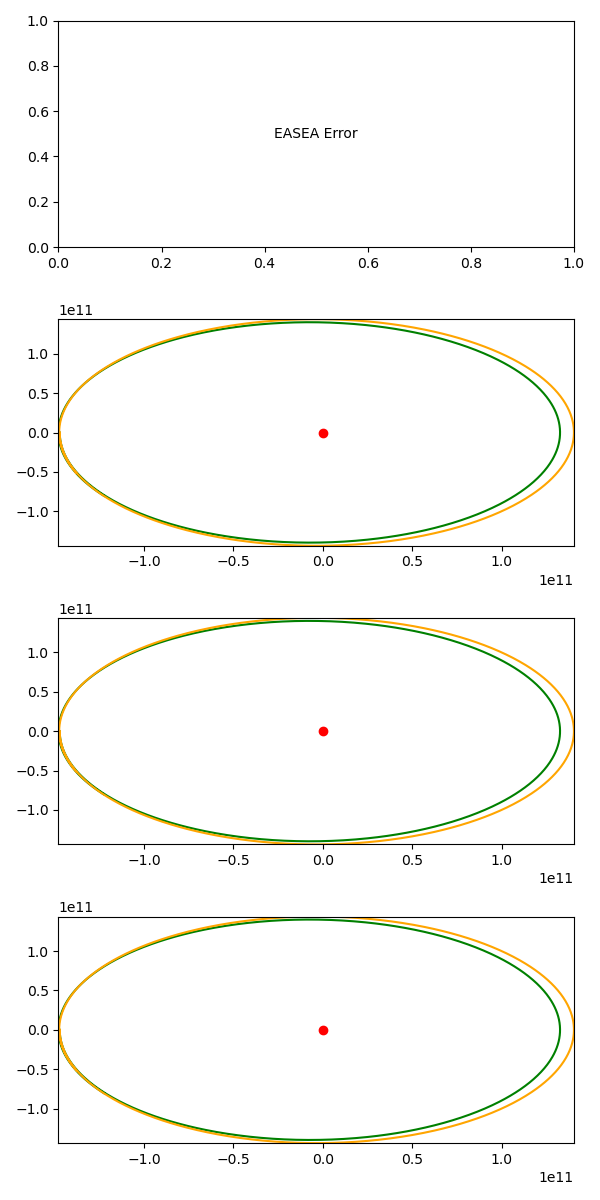
\includegraphics[width=0.5\linewidth,scale=.3]{img/sun_mass.png}
    \caption{Earth trajectories depending of the mass of Sun}
\end{wrapfigure}

\begin{table}[H]
    \begin{tabular}{lllll}
    Number of generations & 60 \\
    Population size & 100 \\
    Offspring size & 100\% \\
    Mutation probability & 0.2 \\
    Mutation variation rate & 0.05
    \end{tabular}
    \caption{Parameters used to find the mass of Sun}
\end{table}

\subsection{Mass of Earth}
We did not managed to find Earth's mass using evolutionnary algorithm as this quantity does not appear in the equations defining Earth's trajectory around Sun. Nonetheless, we have a couple ideas regarding how we could achieve this.\\
The first being to simply change the referential: use the geocentric referential in order to study the movement of Sun. If we only consider those two planets (Earth and Sun) then their movements are relative to each other, that is to say: Earth is orbiting Sun and Sun is also orbiting Earth. In that case, we can can estimate the mass of Earth exactly the same way as we did in the previous part for the mass of Sun.\\
Another way to get to that result would be to study those two celestial bodies in a referential centered on the center of Sun's trajectory. But in this case, we would have to study the movement of Earth is a non-galilean referential which is clearly out of the scope of this study.

\subsection{Speed of Earth at Perihelion}
% \clearpage
\begin{wrapfigure}{R}{0.5\textwidth}
    \center
    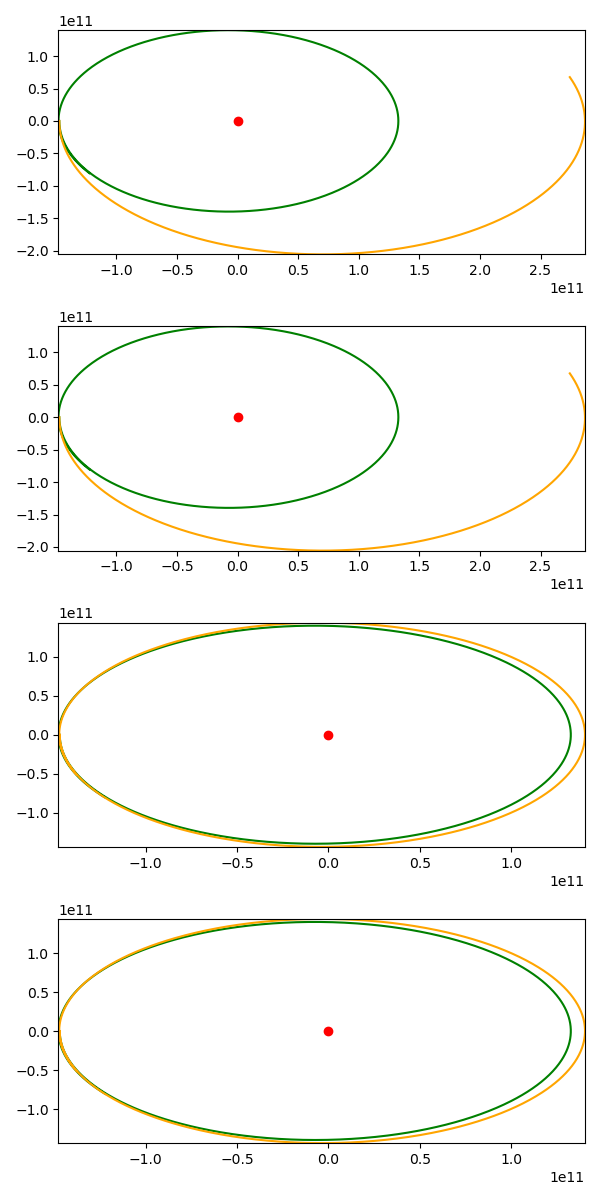
\includegraphics[width=0.5\linewidth,scale=.3]{img/earth_speed.png}
    \caption{Earth trajectories depending of the speed of Earth at the perihelion}
\end{wrapfigure}

In order to find the speed of planet Earth at the perihelion we apply the same steps as before: initialisation, crossover, mutation and evaluation. Unless this time we have to change a couples of values. As the speed of Earth in radian per second is so little, it is not well handled by our program (ie: assimilated to zero). To combat that, we simply consider the speed in radian per day leading to values that can properly be handled by computers. This implies also converting the gravitationnal constant and our sampling step to fit the new unit scale.

\begin{table}
    \begin{tabular}{lllll}
    Number of generations & 100 \\
    Population size & 150 \\
    Offspring size & 100\% \\
    Mutation probability & 0.2 \\
    Mutation variation rate & 0.05
    \end{tabular}
    \caption{Parameters used to find the speed of Earth at the perihelion}
\end{table}